\documentclass{beamer}
\usepackage{graphicx}
\usepackage{algorithm2e}
\usepackage{amsmath,amssymb}
\usepackage{color, colortbl}
\usepackage{qtree}

%%% Beamer Theme %%%
\usetheme{JuanLesPins}
\usecolortheme{beaver}
\beamertemplatenavigationsymbolsempty
\renewcommand\mathfamilydefault{\rmdefault}
%%%

\setlength{\parindent}{0.0cm}

\date{12 March 2012}
\author{Jeremy Mayeres, Charles Newton, Peter Tonner}
\title{Facilitating Large-Scale Graph Searches with Lock-Free Pairing Heaps}

\begin{document}
\maketitle

\begin{frame}{Project Overiew}
  \begin{itemize}
    \item We are constructing a lock-free version of a Pairing heap (a self-balancing heap.)
    \item Pairing heaps have an efficient \texttt{decreaseKey} implementation
      (near-constant performance) that allow you to decrease the value in a heap without
      reinserting it.
    \item This improves the asymptotic performance of certain algorithms (e.g., Dijkstra's algorithm.)
    \item We are comparing our heap against Skipqueues (a priority queue backed with a Skiplist.)
  \end{itemize}
\end{frame}

\begin{frame}{Dijkstra's Algorithm}
  \begin{block}{Single-Source Shortest Path Problem}
    In a weighted graph $G=(V,E)$, find the shortest path from a target
    vertex $v \in V$ to all other vertices in the graph.
  \end{block}
  \begin{itemize}
    \item Push every node in a graph into a priority queue (PQ.) In the PQ, 
      each node is weighted by current information we have about their distance.
    \item Initially, all nodes have a distance of $\infty$, except the target
      node, which has a distance of $0$.
    \item Dynamic programming approach: Inductively build up our shortest routes.
      \begin{itemize}
        \item Pop off the node on the PQ with the smallest distance. (The shortest path from the source to this
          node is finished.)
        \item Update the weights in the PQ with the distances emanating from the popped node.
      \end{itemize}
    \end{itemize}
\end{frame}

\begin{frame}{Skiplists}
  \vspace{-0.2cm}
  \begin{itemize}
    \item Created by Bill Pugh.\footnote{Pugh, ``Skiplists: A Probabilistic Alternative to Balanced Trees,'' 1990.}
    \item Skiplists are constructed from a hierarchy of linked lists with the \textit{Skiplist property}:
      the set of elements contained in level $i$ is a subset of all the levels below it.
    \item Links allow you to do a binary search (``skip'' around.)
    \item The height of an element is random. The probability of
      a node having a height of $i \geq 0$ is $2^{-i}$.
    \item Time complexity of operations are probabilistically the same as for a binary search tree, but
      $\mathcal{O}(n)$ in the worst case.
  \end{itemize}
  \begin{center}
    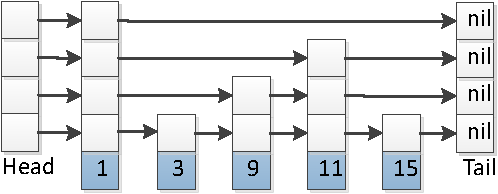
\includegraphics[scale=0.75]{img/skiplist-crop.pdf}
  \end{center}
\end{frame}

\begin{frame}{Skiplists (Search)}
  \begin{itemize}
    \item For each level, move right until you run into a node greater than your target. Then, from
      this point, move right on the next lowest level, and repeat.
    \item Likely runs in $\mathcal{O}(\log n)$ time.
    \item Head / tail nodes have values of $-\infty$ and $\infty$, respectively.
  \end{itemize}
  \begin{center}
    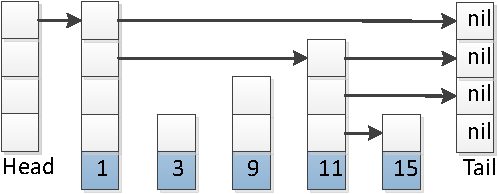
\includegraphics[scale=0.75]{img/skiplistSearch15-crop.pdf}
  \end{center}
\end{frame}

\begin{frame}{Next and Previous Windows}
  \begin{itemize}
    \item A useful abstraction to make is the set of all pointers
      related to a given node. (Aggregate all the pointers related to one node.)
    \item $\mathtt{prev[}i\mathtt{]} \rightarrow$ the node in level $i$ pointing to the target node.
    \item $\mathtt{next[}i\mathtt{]} \rightarrow$ the node the target node points to at level $i$.
    \item Use the search process to construct these sets.
  \end{itemize}
  \begin{center}
    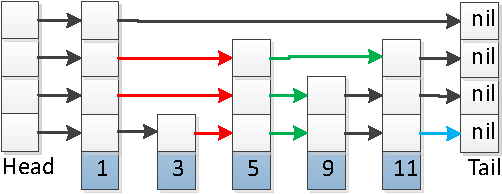
\includegraphics[scale=0.75]{img/skiplistInsert5-crop.pdf}
  \end{center}
\end{frame}

\begin{frame}{Skiplists (Insertion)}
  \begin{itemize}
    \item Insertion: Find the location the target should be at.
      Set all of the node's next pointers to $\mathtt{next[}i\mathtt{]}$ and set
      the next pointers at each $\mathtt{prev[}i\mathtt{]}$ to the new node.
  \end{itemize}
  \begin{center}
    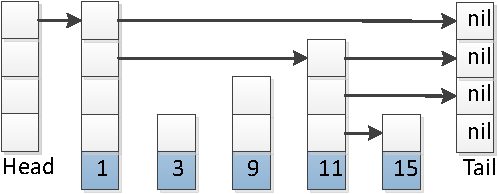
\includegraphics[scale=0.75]{img/skiplistSearch15-crop.pdf}
  \end{center}
  \begin{center}
    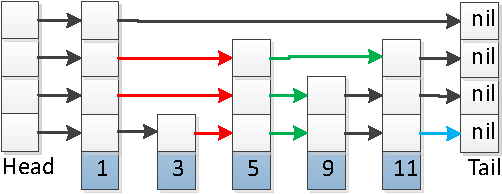
\includegraphics[scale=0.75]{img/skiplistInsert5-crop.pdf}
  \end{center}
\end{frame}

\begin{frame}{Skiplists (Deletion)}
  \begin{itemize}
    \item Deletion: Set all of the next pointers in $\mathtt{prev[}i\mathtt{]}$ 
      equal to $\mathtt{next[}i\mathtt{]}$.
  \end{itemize}
  \begin{center}
    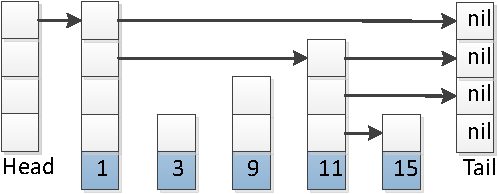
\includegraphics[scale=0.75]{img/skiplistSearch15-crop.pdf}
  \end{center}
  \begin{center}
    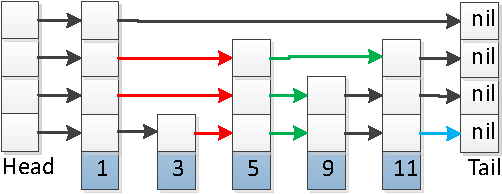
\includegraphics[scale=0.75]{img/skiplistInsert5-crop.pdf}
  \end{center}
\end{frame}

\begin{frame}{Lock-free Skiplists}
  \begin{itemize}
    \item Created by Herlihy, Lev, and Shavit.\footnote{Herlihy, Lev, Shavit, ``A Lock-Free Concurrent Skiplist with Wait-Free Search,'' 2007.}
    \item Instead of linked lists at each level, we use lock-free linked lists.
    \item We lose the Skiplist property. (Levels aren't necessarily subsets of each other.) In particular,
      this means we need to always verify a node is in the lowest level.
  \end{itemize}
\end{frame}

\begin{frame}{Lock-free Skiplists}
  \begin{itemize}
    \item Instead of linked lists at each level, we use lock-free linked lists.
    \item Linearization point: membership is defined at the lowest level of the Skiplist.
    \item We lose the Skiplist property. (Levels aren't necessarily subsets of each other.) In particular,
      this means we need to always verify a node is in the lowest level.
  \end{itemize}
\end{frame}

\begin{frame}{Lock-Free Skiplists (Insertion)}
  \begin{itemize}
    \item Construct the $\mathtt{prev[}i\mathtt{]}$ and $\mathtt{next[}i\mathtt{]}$ sets.
    \item Set all of the node's next pointers to $\mathtt{next[}i\mathtt{]}$.
    \item If we can CAS the node into the bottom level, continue. Otherwise, something changed, and
      restart (reconstruct $\mathtt{prev[}i\mathtt{]}$ and $\mathtt{next[}i\mathtt{]}$).
    \item Next, CAS all $\mathtt{prev[}i\mathtt{]}$ to the new node. If a CAS fails, reconstruct
      $\mathtt{prev[}i\mathtt{]}$.
  \end{itemize}
\end{frame}

\begin{frame}{Lock-Free Skiplists (Deletion)}
  \begin{itemize}
    \item Pointers are atomically \textit{markable}.
      \begin{itemize}
        \item In C / C++, steal a bit from the pointer.
        \item In Java, use \texttt{AtomicMarkableReference}.
      \end{itemize}
    \item Construct the $\mathtt{prev[}i\mathtt{]}$ and $\mathtt{next[}i\mathtt{]}$ sets.
    \item For each pointer in our target node, mark them as deleted.
  \end{itemize}
\end{frame}

\begin{frame}{Optimized \texttt{decreaseKey} for Lock-Free Skiplists}
  \begin{itemize}
    \item Currently, to implement a \texttt{decreaseKey} for Skiplists, we need to
      do two $\mathcal{O}(\log n)$ operations (one insert and one delete.)
    \item We can optimize this in some cases by removing redundant work: reuse the
      $\mathtt{prev[}i\mathtt{]}$ set as a starting point for the next insertion.
  \end{itemize}
\end{frame}

\begin{frame}{Pairing Heaps}
  \begin{itemize}
    \item Pairing Heaps were introduced by Fredman and Tarjan\footnote{``The Pairing heap: a new form of self-adjusting heap,'' Fredman, Sedgewick, Sleator, and Tarjan, Algorithmica (1986).} as a simplification of Fibonacci heaps.
     \begin{itemize}
        \item Fibonacci heaps have a $\mathcal{O}(1)$ \texttt{decreaseKey} operator, but require complicated rebalancing.
      \end{itemize}
    \item \texttt{decreaseKey} runs in $2^{\mathcal{O}(\sqrt{\log \log n})}$ time.
        \begin{itemize}
          \item In practice, constant time. E.g., for a graph with a billion edges, $2^{\sqrt{\log \log 10^9}} = 3.34$.
        \end{itemize}
      \item Pairing heaps have better performance than Fibonacci heaps on reasonably-sized graphs.\footnote{``On the Efficiency of Pairing Heaps and Related Data Structures,'' Michael Fredman, Journal of the ACM, 1999.}
  \end{itemize}
\end{frame}

\begin{frame}{Pairing Heaps}
  \begin{itemize}
    \item Pairing Heaps were introduced by Fredman and Tarjan.
    \item Each node is a sub-heap
    \item The parent of any node has key smaller than the child node
    \item Each node has a left pointer to its first child, and a right pointer to its sibling
    \item Like \texttt{decreaseKey}, other operations run quickly as well
    	\begin{itemize}
    	\item \texttt{meld}: $\mathcal{O}(1)$
    	\item \texttt{findMin}: $\mathcal{O}(1)$
    	\item \texttt{insert}: $\mathcal{O}(1)$
    	\end{itemize}
    \item \texttt{delete} and \texttt{deleteMin} run in $\mathcal{O}(\log n)$ amortized time     
  \end{itemize}
\end{frame}

\begin{frame}{Pairing Heaps: Melding Two Heaps}
  \begin{itemize}
    \item To \texttt{meld} two heaps, compare their roots and add the root
      as a child of the smaller root.
    \item \texttt{meld} is the core operator for Pairing heaps.
    \item Example: Melding two min-heaps together (root 3 and root 5)
  \end{itemize}
  \begin{figure}
	  \Tree [.3 [.5 \qroof{T_1}.10 [.12 \qroof{T_2}.19 \qroof{T_3}.20 ] \qroof{T_4}.34 ] !{\qframesubtree} [.25 [.19 \qroof{T_5}.20 \qroof{T_6}.21 ] \qroof{T_7}.42 ] ]
	  \label{fig:meld}
  \end{figure}
\end{frame}

\begin{frame}{Pairing Heaps: \texttt{insert}}
  \begin{itemize}
    \item To insert a new element into a pairing heap, construct a
      trivial heap containing only that element and \texttt{meld}
      this to the root.
    \item (The root of the heap will change if the new element is lower.)
  \end{itemize}
\end{frame}

\begin{frame}{Pairing Heaps: \texttt{decreaseKey}}
  \begin{itemize}
    \item Change the value of a node in the pair heap (e.g. updating the minimum distance to a node in Dijkstra's algorithm)
    \item If new value is still greater than parent node value, change in place
    \item Alternatively, remove node from heap, \texttt{insert} node with new value into heap
  \end{itemize}
\end{frame}

\begin{frame}{Pairing Heaps: \texttt{deleteMin}}
  \begin{itemize}
    \item \texttt{deleteMin} removes the root node of a Pair Heap (e.g. pop off node with shortest distance in Dijkstra's algorithm)
    \item The root of the heap is first removed
    \item The heap property must then be restored by finding a new root
    \item Build pairs of heaps from the children of the root
    \item \texttt{meld} each resultant heap from right-to-left.
  \end{itemize}
\end{frame}

\begin{frame}{Pairing Heaps: \texttt{deleteMin} Pairing Operation}
  \begin{itemize}
  \item The root of the tree has $n$ sub-trees $H_1, H_2, \dots, H_n$, each with their own individual roots. 
  \item For each tuple in the set $\{(H_1, H_2), (H_3, H_4), \dots, \allowbreak (H_{n-1}, H_n)\}$, we meld the two heaps together to form $\{H'_1, \dots, \allowbreak H'_m\}$.	
   \item Perform a right-iteration (similar to foldr) of \texttt{meld} over these $m=\frac{n}{2}$ (or $m=\frac{n-1}{2} + 1$) heaps to construct a newly rebalanced pairing heap
   \item $H'$:
	\begin{equation*}
	  H' = \mathtt{meld}(H'_1, \mathtt{meld}(H'_2, \dots \mathtt{meld}(H'_{m-1}, H'_m) \dots ))
	\end{equation*}
  \end{itemize}
\end{frame}

\begin{frame}{Pairing Heaps: \texttt{deleteMin} Example}
  \begin{itemize}
    \item Example of the \texttt{deleteMin} operation
  \end{itemize}
  \begin{figure}
	  \begin{enumerate}
	   \item[(a)] \Tree [.7 [20 15 8 9 42 ] ] 
	   \item[(b)] \Tree [20 15 8 9 42 ]
	   \item[(c)] \Tree [.15 20 ]
		      \Tree [.8 9 ]
		      \Tree [.42 ]
	   \item[(d)] \Tree [.15 20 ]
		      \Tree [.8 42 9 ]
	   \item[(e)] \Tree [.8 [.15 20 ] 42 9 ]
	  \end{enumerate}
    \caption{Calling \texttt{deleteMin} on a Pairing heap (a). The root is removed (b) and the children are melded in pairs (c), and then the pairs themselves are melded in right-to-left order (d-e). Note that the resulting heap (e) is more balanced than (a).}
    \label{fig:deletemin}
  \end{figure}
\end{frame}

%\begin{frame}{Pairing Heaps: \texttt{deleteMin}}
%  \begin{itemize}
%    \item Pairing heaps have a two-step deleteMin operator.
%  \end{itemize}
%  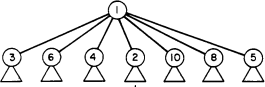
\includegraphics[scale=1.0]{img/deleteMin1.png}
%\end{frame}

%\begin{frame}{Pairing Heaps: \texttt{deleteMin}}
%  \begin{itemize}
%    \item After removing the root, \texttt{meld} each pair of heaps.
%  \end{itemize}
%  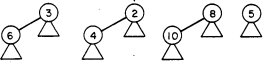
\includegraphics[scale=1.0]{img/deleteMin2.png}
%\end{frame}

%\begin{frame}{Pairing Heaps: \texttt{deleteMin}}
%  \begin{itemize}
%    \item \texttt{meld} each resultant heap from right-to-left.
%  \end{itemize}
%  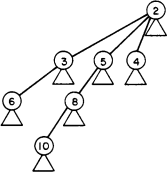
\includegraphics[scale=1.0]{img/deleteMin3.png}
%\end{frame}

\begin{frame}{Parallelizing Dijkstra's Algorithm}
  \begin{itemize}
  \item To simplify our Pairing heap implementation, we will only
    consider function interleavings that can occur when the heap is used
    for Dijkstra's algorithm.
  \item For Dijkstra's algorithm, we pop the minimum off the PQ (\texttt{deleteMin})
    and call \texttt{decreaseKey} on the node's neighbors.
  \item If \texttt{decreaseKey} produces new heap minima, this will affect
    future calls to \texttt{deleteMin}
  \item For this reason, we assume that calls to \texttt{decreaseKey} and \texttt{deleteMin}
    never intersect.
  \end{itemize}
\end{frame}

\begin{frame}{Lock-Free Pairing Heaps: Overview}
  \begin{itemize}
    \item Modify the list of sub-heaps to be a lock-free list of subheaps.
    \item We have identified an easy linearization point for \texttt{insert} and \texttt{deleteMin}:
      a node is considered in-place when the root is updated (CAS'd into place.)
      \begin{itemize}
        \item But, what if the new node is inserted as a subheap of the current root?
        \item We create a copy of the root to avoid this issue.
      \end{itemize}
    \item Each node reference is updateable through a CAS operation
    \item In Java: \texttt{AtomicReference}
    \item Operations requiring linking nodes together use CAS loops
    \item Operations requiring node removal additionally use time stamps
    \item Build more complex lock-free operations from simpler ones
  \end{itemize}
\end{frame}

\begin{frame}{Lock-Free Pairing Heaps}
  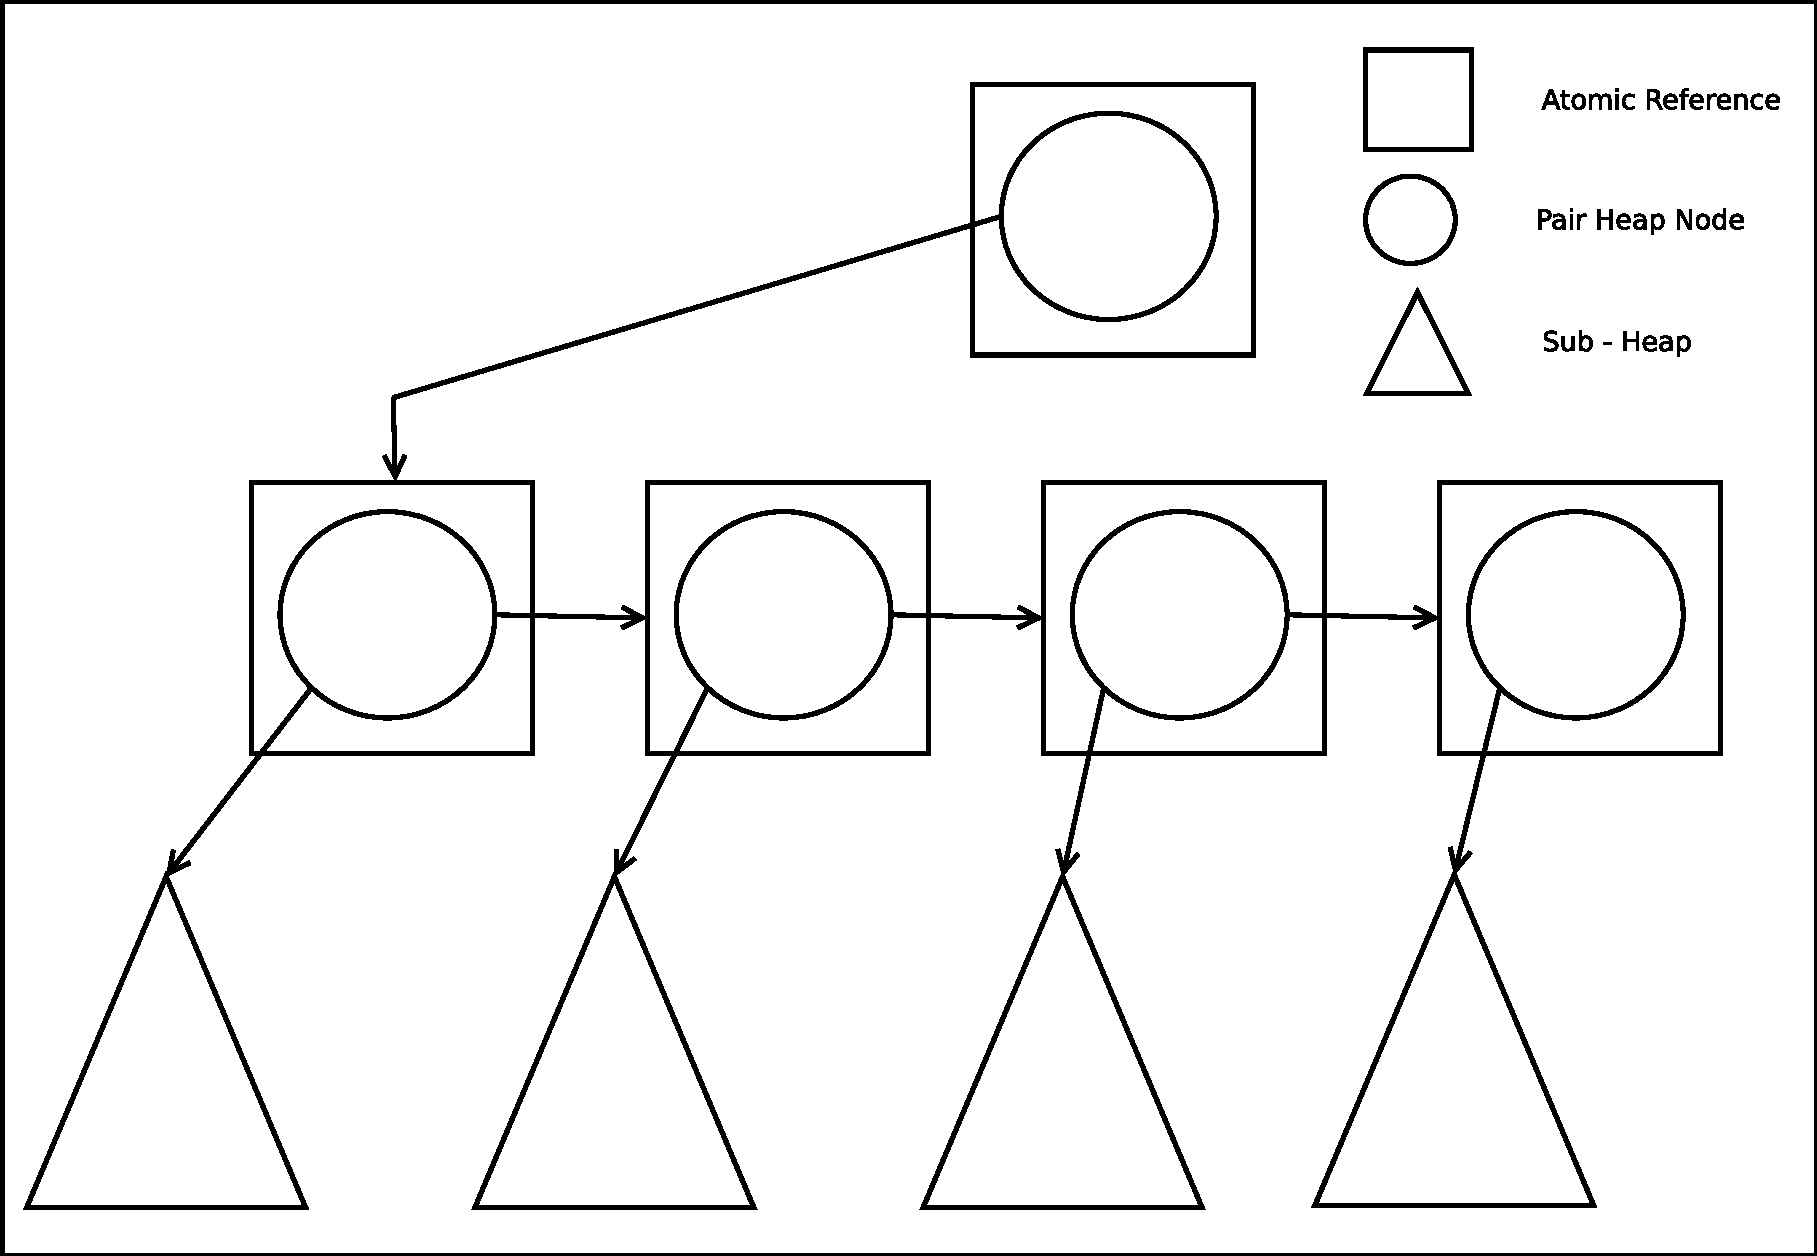
\includegraphics[scale=.350]{img/pairheapLockFree.pdf}
\end{frame}

\begin{frame}{Lock-Free Pairing Heaps: \texttt{insert} an element}
  \begin{itemize}
    \item Recall the insertion procedure: create a trivial heap containing only that
      element and \texttt{meld} it to the root.
    \item Lock-free \texttt{insert}:
      \begin{itemize}
        \item Create a copy of the root, but the root and its copy share the same
          list of subheaps (this avoids an $\mathcal{O}(n)$ copy.)
        \item Meld the new heap with the copy of the root.
        \item Try to CAS the new root as the root of the heap.
        \item If CAS succeeds, we're done.
        \item If CAS fails, delete the subheap list changes and retry.
      \end{itemize}
    \end{itemize}
\end{frame}

\begin{frame}{Lock-Free Pairing Heaps: \texttt{decreaseKey}}
  \begin{itemize}
    \item Main observation: If Dijkstra's algorithm is run on a graph with
      exactly $0$ or $1$ edge between each node, calls to \texttt{decreaseKey}
      will be unique (per iteration.)
    \item \textbf{Case 1}: If the parent is still smaller than the node, just decrease the value.
      \begin{itemize}
        \item We know that this node won't replace the root, since the parent is larger.
          An interleaved call to change the parent can only decrease its value.
      \end{itemize}
    \item \textbf{Case 2}: If we're trying to decrease the value of the root, copy the root (as before),
      decrease its value, and try to CAS the new root into place. After a CAS fails, check if
      we are still trying to decrease the root and repeat if so.
    \item \textbf{Case 3}: The node is now smaller than its parent, violating the heap invariant. Immediately remove
      the node from the parent's list of subheaps. Next, follow the same procedure as \texttt{insert}.
  \end{itemize}
\end{frame}

\begin{frame}{Lock-Free \texttt{deleteMin}}
    \begin{itemize}
    	\item Requires the removal of root node and restructuring of heap architecture
    	\item Root reference and timestamp will be used to update the heap
    \end{itemize}
\end{frame}


\begin{frame}{Practical Considerations}
  \begin{itemize}
    \item Skiplists are extremely concurrent, but require
      two $\mathcal{O}(\log n)$ operations to implement \texttt{decreaseKey}. Also,
      operations require many pointer updates.
    \item Pairing heaps have a near-constant \texttt{decreaseKey} implementation and fewer
      pointer updates per call, but
      every operation is contending for the same location in memory (every thread contends for the root.)
  \end{itemize}
\end{frame}

\begin{frame}{Experimentation}
  \begin{itemize}
    \item Run Dijkstra's algorithm on various large graphs
      (both randomly generated and real-world, e.g, from Harvard's Human Interactome Database.)
    \item Compare the time Dijkstra's algorithm takes for a Skiplist-backed implementation vs. a lock-free Pairing heap.
    \item Run experiments with varying numbers of threads.
  \end{itemize}
\end{frame}

\end{document}
